\begin{figure}[t]
	\centerline{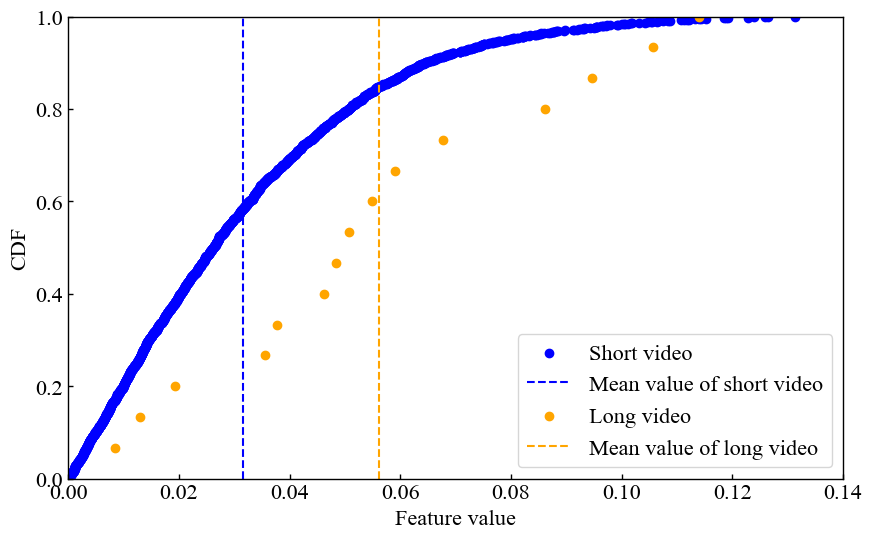
\includegraphics[width=\linewidth]{img/result/feature_distribution/CDF/CDF_plot_diff_zncc_50_dx.png}}
	\caption{CDF of image-based characterizations (50th percentile values) projected along x-axis}
	\label{cdf_ZNCC50_dx}
\end{figure}

\begin{figure}[t]
	\centerline{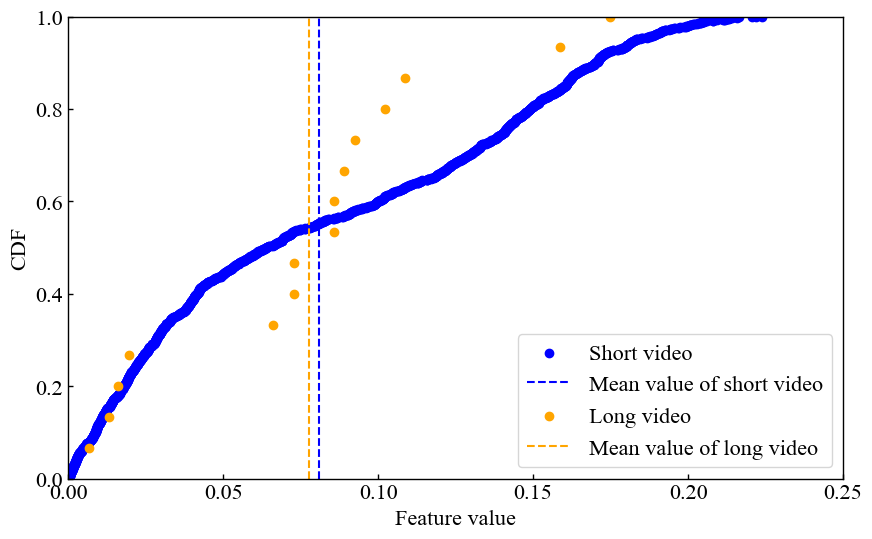
\includegraphics[width=\linewidth]{img/result/feature_distribution/CDF/CDF_plot_diff_zncc_50_dy.png}}
	\caption{CDF of image-based characterizations (50th percentile values) projected along y-axis}
	\label{cdf_ZNCC50_dy}
\end{figure}

\begin{figure}[t]
	\centerline{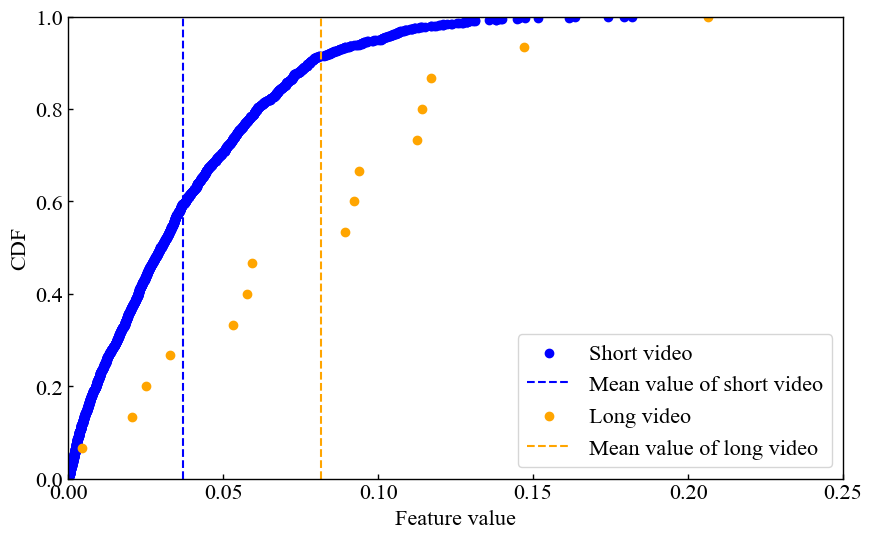
\includegraphics[width=\linewidth]{img/result/feature_distribution/CDF/CDF_plot_diff_zncc_50_dz.png}}
	\caption{CDF of image-based characterizations (50th percentile values) projected along z-axis}
	\label{cdf_ZNCC50_dz}
\end{figure}

\begin{figure}[t]
	\centerline{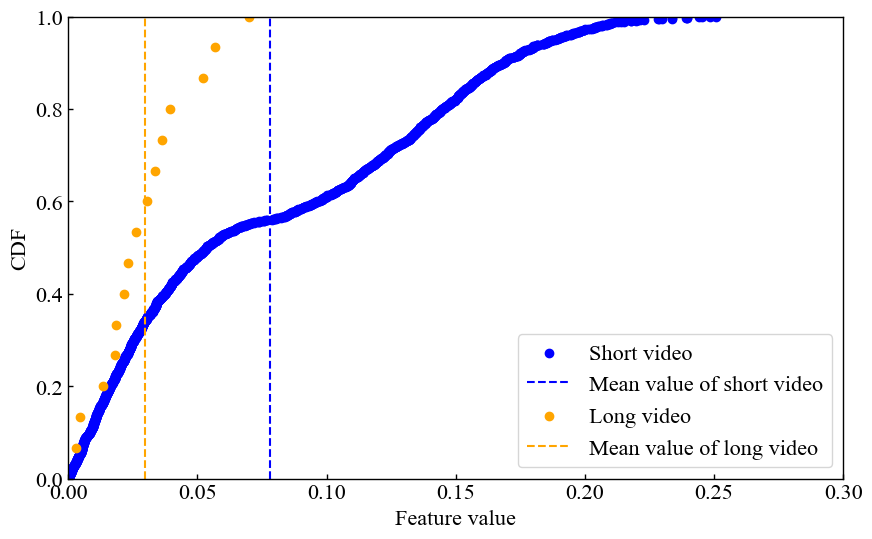
\includegraphics[width=\linewidth]{img/result/feature_distribution/CDF/CDF_plot_diff_zncc_90_dx.png}}
	\caption{CDF of image-based characterizations (90th percentile values) projected along x-axis}
	\label{cdf_ZNCC90_dx}
\end{figure}

\begin{figure}[t]
	\centerline{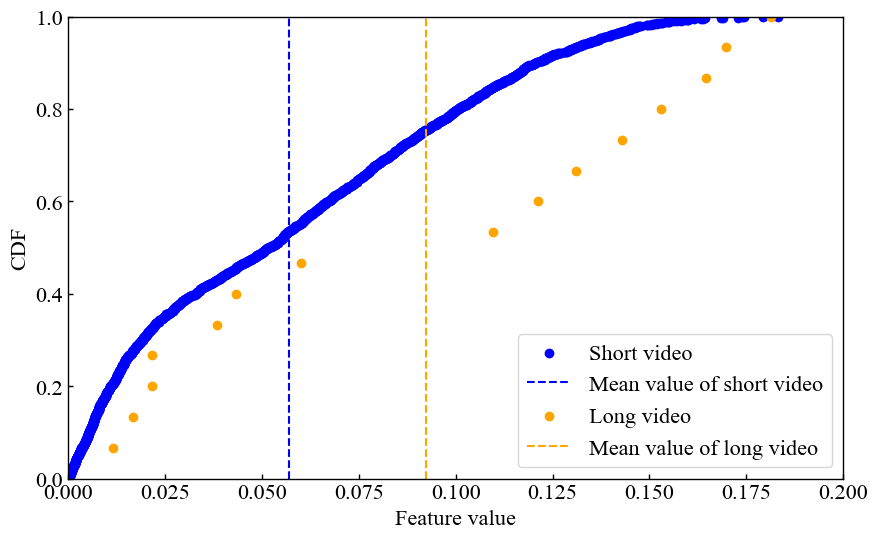
\includegraphics[width=\linewidth]{img/result/feature_distribution/CDF/CDF_plot_diff_zncc_90_dy.png}}
	\caption{CDF of image-based characterizations (90th percentile values) projected along y-axis}
	\label{cdf_ZNCC90_dy}
\end{figure}

\begin{figure}[t]
	\centerline{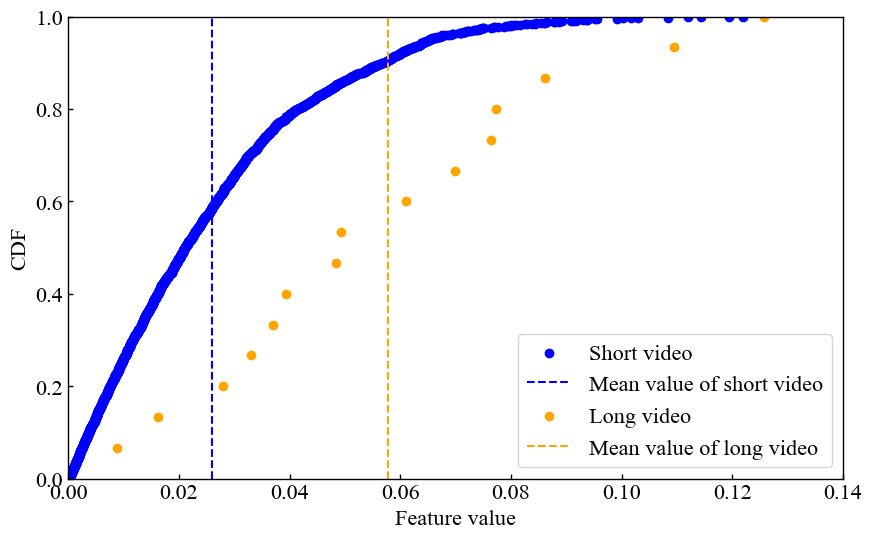
\includegraphics[width=\linewidth]{img/result/feature_distribution/CDF/CDF_plot_diff_zncc_90_dz.png}}
	\caption{CDF of image-based characterizations (90th percentile values) projected along z-axis}
	\label{cdf_ZNCC90_dz}
\end{figure}

\begin{figure}[t]
	\centerline{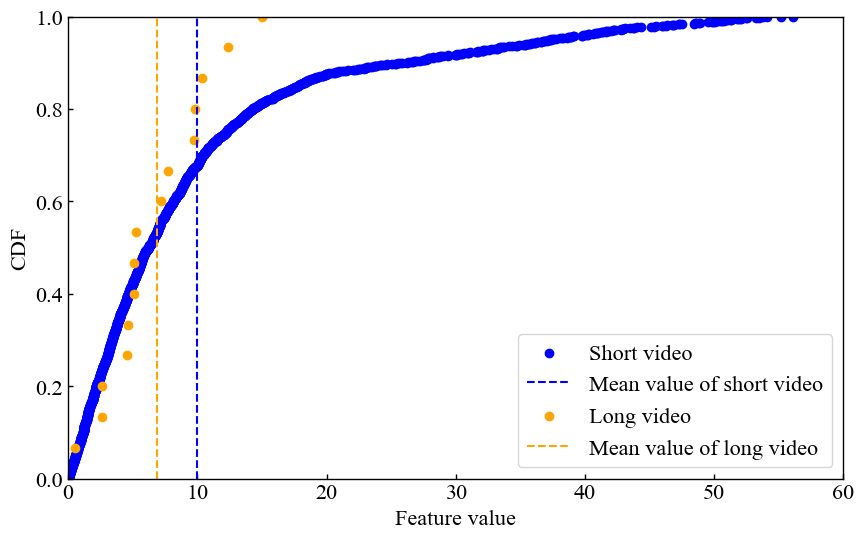
\includegraphics[width=\linewidth]{img/result/feature_distribution/CDF/CDF_plot_diff_centoroid_50.png}}
	\caption{CDF of centroid characterization (50th percentile values)}
	\label{cdf_centroid50}
\end{figure}

\begin{figure}[t]
	\centerline{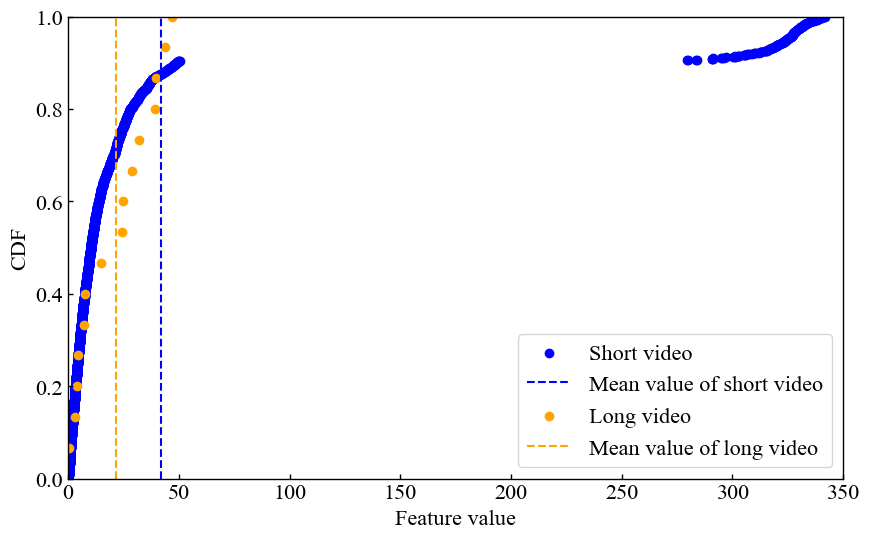
\includegraphics[width=\linewidth]{img/result/feature_distribution/CDF/CDF_plot_diff_centoroid_90.png}}
	\caption{CDF of centroid characterization (90th percentile values)}
	\label{cdf_centroid90}
\end{figure}

% 
This section discusses in terms of distribution of features, the accuracy of inference from short-video data for long-video data.
% 
Figs.~\ref{cdf_ZNCC50_dx} to \ref{cdf_centroid90} show the cumulative distribution function (CDF) of the two datasets.
% 
The vertical axis shows the CDF, while the horizontal axis shows real values of features. 

% 
Fig.~\ref{cdf_ZNCC50_dx} shows the CDF of the 50th percentile values of the feature values reflecting variation in the front-back direction of the body. 
% 
The CDF showed a similar trend in the two sets of data. 
% 
The shapes of the graphs in both cases showed a gentle upward slope to the right, and the range of feature values exhibited a similar trend.
% 
The magnitude of the feature values tended to be larger in the test data compared with the means. 
% 
The distribution's scatter indicated a small standard deviation of about 0.03 in the test data, suggesting minimal variance in the values between the two datasets.

% 
Fig.~\ref{cdf_ZNCC50_dy} shows the CDF of the 50th percentile values of the feature values reflecting variation in the left-right direction of the body. 
% 
The CDF showed a different trend in both datasets. 
% 
The shapes of the graphs differed for each. 
% 
The shape of the graph for the training data indicated a gentle upward slope to the right.
% 
The distribution of the graph was limited to a narrow range, with overlap observed in certain ranges of the CDF.
% 
The magnitude of the feature values showed no significant difference in the two set of data based on a comparison of the means. 
% 
The scatter of the distribution showed a tendency toward larger variability with a standard deviation of about 0.05 for the test data.

% 
Fig.~\ref{cdf_ZNCC50_dz} shows the CDF of the 50th percentile values of the feature values reflecting the variation in the vertical direction of the body. 
% 
The CDF showed different trends in the two sets of data. 
% 
The shapes of the graphs differed for each. 
% 
The shape of the graph for the training data indicated a gentle upward slope to the right.
% 
The graph of the test data showed a tendency for certain feature values to be concentrated in a narrow range.
% 
The magnitude of the feature values tended to be larger in the test data compared with the means. 
% 
The scatter of the distribution tended to be smaller in the test data. 

% 
Fig.~\ref{cdf_ZNCC90_dx} shows the CDF of the 90th percentile values of the feature values reflecting the variation in the front-back direction of the body. 
% 
The CDF showed different trends in the two sets of data. 
% 
The shapes of the graphs differed for each. 
% 
The shape of the graph for the training data indicated a gentle upward slope to the right.
% 
The shape of the graph for the test data showed a steep gradient.
%
The magnitude of the feature values tended to be larger in the training data compared with the means. 
% 
The scatter of the distribution tended to be smaller in the test data.

% 
Fig.~\ref{cdf_ZNCC90_dy} shows the CDF of the 90th percentile values of the feature values reflecting the variation in the left-right direction of the body. 
% 
The CDF showed a similar trend in the two sets of data. 
% 
The shapes of the graphs in both cases showed a gentle upward slope to the right, and the range of feature values exhibited a similar trend.
% 
The magnitude of the feature values tended to be larger in the test data compared with the means. 
% 
The scatter of the distribution showed a tendency to be larger in the training data compared with the test data.

% 
Fig.~\ref{cdf_ZNCC90_dz} shows the CDF of the 90th percentile values of the feature values reflecting the variation in the vertical direction of the body. 
%
The CDF showed different trends in the two sets of data. 
% 
The shapes of the graphs differed for each. 
% 
The shape of the graph for the training data indicated a gentle upward slope to the right.
% 
The distribution of graph of the test data was limited to a narrow range.
% 
The magnitude of the feature values tended to be larger in the test data compared with the means. 
% 
The scatter of the distribution tended to be small for the training data and large for the test data. 

% 
Fig.~\ref{cdf_centroid50} shows the CDF of the 50th percentile values of the feature values reflecting the variation of the head center of gravity. 
%
The CDF showed different trends in the two sets of data. 
% 
The shapes of the graphs were different for each. 
% 
The shape of the graph for the training data showed a gentle upward slope. 
% 
The distribution of graph of the test data was limited to a narrow range.
%
The magnitude of the feature values tended to be larger in the training data compared with the means. 
% 
The scatter of the distribution was small in the test data with a standard deviation of approximately 3.84. 

%
Fig.~\ref{cdf_centroid90} shows the CDF of the 90th percentile values of the feature values reflecting the variation of the head center of gravity. 
% 
The CDF showed different trends in the two sets of data. 
% 
The shape of the graphs were different for each. 
% 
The shape of the graph for the training data showed a steep gradient, with outliers observed above a CDF of approximately 0.9.
% 
The shape of the graph for the test data showed a steep gradient. 
% 
The magnitude of the feature values tended to be larger in the training data compared with the means. 
% 
The scatter of the distribution was small in the test data with a standard deviation of approximately 3.84. 

%
We investigated the impact of video duration differences on estimation by comparing the CDFs and analyzing feature distribution trends.
%
The analysis revealed that there were differences in feature distributions between short and long video data.
%
Notably, the CDFs for features reflecting variations in the vertical movement of the body and the center of gravity of the head showed a significant discrepancy due to video duration, as illustrated in 
%
Figs.~\ref{cdf_ZNCC50_dz}, \ref{cdf_ZNCC90_dz}, \ref{cdf_centroid50}, and \ref{cdf_centroid90}.
%
These differences in distribution trends suggest the presence of feature distribution differences between short-video data and long-video data.